\documentclass[11pt,a4paper]{article}
\usepackage[utf8]{inputenc}
\usepackage[vietnamese]{babel}
\usepackage{amsmath,amssymb}
\usepackage[version=4]{mhchem}
\usepackage{geometry}
\geometry{top=1.5cm,bottom=1.2cm,left=1.4cm,right=1.4cm,headheight=28pt,headsep=12pt,footskip=18pt}
\usepackage{graphicx}
\usepackage{xcolor}
\usepackage{tabularx}
\usepackage{array}
\usepackage{tikz}
\usepackage{fancyhdr}
\usepackage{enumitem}

\definecolor{hfRed}{HTML}{D32F2F}
\definecolor{hfGreen}{HTML}{8BC390}
\definecolor{mainGreen}{HTML}{2E7D32}

\usepackage{ex_test}

\pagestyle{fancy}
\fancyhf{}
\renewcommand{\headrulewidth}{0.75pt}
\renewcommand{\headrule}{\hbox to\headwidth{\color{hfGreen}\leaders\hrule height \headrulewidth\hfill}}
\renewcommand{\footrulewidth}{0.75pt}
\renewcommand{\footrule}{\hbox to\headwidth{\color{hfGreen}\leaders\hrule height \footrulewidth\hfill}}

\fancyhead[L]{\small\itshape\color{hfRed}Tài liệu lưu hành nội bộ}
\fancyhead[R]{\small\color{hfRed}Thầy \textbf{TRẦN VĂN THẠNH} - 0777.470.803}

\fancyfoot[L]{\footnotesize\itshape\color{hfRed}CS1: 6/15 Nguyễn Hoàng, P. Kim Long, TP Huế \quad|\quad CS2: 24 Đặng Thái Thân, TP Huế}
\fancyfoot[R]{\small\textbf{\color{hfRed}Trang \thepage}}

\setlength{\parindent}{0pt}
\setlength{\parskip}{1.5pt}

\begin{document}

\begin{minipage}[t]{0.45\textwidth}
\textbf{SỞ GIÁO DỤC VÀ ĐÀO TẠO}\\
\textbf{TRƯỜNG THPT}\\
\textit{ĐỀ CHÍNH THỨC}\\
\textit{(Đề gồm 4 phần, 4 trang)}
\end{minipage}
\hfill
\begin{minipage}[t]{0.52\textwidth}
\raggedleft
\textbf{\color{hfRed}KIỂM TRA GIỮA KỲ 1 -- NĂM HỌC 2026 -- 2027}\\
\textbf{MÔN: HÓA HỌC -- KHỐI 10}\\
\textit{Thời gian làm bài: 45 phút (không kể thời gian phát đề)}\\
\textbf{MÃ ĐỀ: 5001}
\end{minipage}

\vspace{3pt}
\noindent
\textit{Họ, tên thí sinh:} \dotfill \textit{Lớp:} \dotfill \textit{SBD:} \dotfill

\vspace{2pt}
\noindent
\textit{\footnotesize (Cho biết nguyên tử khối: H = 1; C = 12; N = 14; O = 16; Na = 23; Mg = 24; Al = 27; P = 31; S = 32; Cl = 35,5; K = 39; Ca = 40; Fe = 56; Cu = 64; Zn = 65; Ga = 69,7; In = 114,8).}

\vspace{2pt}
\noindent
\textbf{\color{mainGreen}PHẦN I. Câu trắc nghiệm nhiều phương án lựa chọn.}\\
\textit{Học sinh trả lời từ câu 1 đến câu 12. Mỗi câu hỏi học sinh chỉ chọn một phương án. (3,0 điểm)}

\Opensolutionfile{ans}[ans-5001-hs]

\begin{ex}
Ứng dụng nào sau đây thể hiện vai trò của hóa học trong lĩnh vực bảo vệ môi trường?
\choice
{Tổng hợp thuốc kháng sinh để điều trị bệnh nhiễm khuẩn.}
{\True Chế tạo vật liệu hấp phụ để loại bỏ ion kim loại nặng trong nước thải nhà máy dệt.}
{Sản xuất xi măng phục vụ xây dựng nhà ở.}
{Sản xuất phân đạm để tăng năng suất cây trồng.}

\end{ex}

\begin{ex}
Năm 2026, một nhóm nghiên cứu khoa học đã tận dụng phụ phẩm của cây cải dầu (bã ép, thân, lá, hoa) để chế tạo màng bao gói thực phẩm phân hủy sinh học. Màng được tạo từ chitosan, chiết xuất phenolic và hạt nano bạc, giúp kéo dài thời gian bảo quản rau quả tươi. Hoạt động nào sau đây thuộc phạm vi nghiên cứu của hóa học?
\choice
{Điều tra thói quen và mức độ sẵn sàng sử dụng bao gói xanh của người tiêu dùng.}
{Khảo sát chi phí sản xuất và khả năng thương mại hóa màng bao gói trên thị trường.}
{Nghiên cứu đặc điểm sinh trưởng của cây cải dầu nhằm nâng cao năng suất thu hoạch.}
{\True Xác định thành phần, cấu trúc của màng và sự biến đổi của màng khi bị phân hủy trong đất.}

\end{ex}

\begin{ex}
Hình vẽ sau mô tả thí nghiệm tìm ra hạt X là một trong những thành phần cấu tạo nên nguyên tử.
\begin{center}
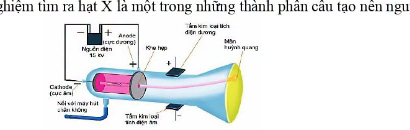
\includegraphics[width=7cm]{images_gk1_10_5001/cau3_ong_phong_tia.png}
\end{center}
Hạt X là
\choice
{proton.}
{neutron.}
{\True electron.}
{neutron và proton.}

\end{ex}

\begin{ex}
Các nguyên tố trong bảng tuần hoàn hiện nay được xếp theo chiều tăng dần của
\choice
{\True điện tích hạt nhân nguyên tử.}
{nguyên tử khối.}
{số neutron.}
{số lớp electron.}

\end{ex}

\begin{ex}
Năm 1911, Rutherford cho chùm hạt $\alpha$ bắn vào một lá vàng rất mỏng và quan sát thấy hầu hết các hạt $\alpha$ đi thẳng qua lá vàng. Kết quả này chứng tỏ
\choice
{hạt nhân nguyên tử mang điện tích âm.}
{nguyên tử không chứa hạt mang điện.}
{electron có khối lượng rất lớn.}
{\True nguyên tử có cấu tạo rỗng.}

\end{ex}

\begin{ex}
Hạt nhân nguyên tử chứa 28 hạt neutron là
\choice
{\ce{^{32}_{16}S}.}
{\True \ce{^{54}_{26}Fe}.}
{\ce{^{58}_{28}Ni}.}
{\ce{^{32}_{15}P}.}

\end{ex}

\begin{ex}
Nguyên tố hóa học là những nguyên tử có cùng
\choice
{số khối.}
{số neutron.}
{số neutron và số proton.}
{\True số proton.}

\end{ex}

\begin{ex}
Phát biểu nào sau đây không đúng?
\choice
{Phân lớp p có nhiều orbital hơn phân lớp s.}
{Số electron tối đa trên phân lớp d gấp năm lần số electron tối đa trên phân lớp s.}
{Số lượng electron tối đa trong một phân lớp luôn là một số chẵn.}
{\True Electron càng ở xa hạt nhân thì có năng lượng càng thấp.}

\end{ex}

\begin{ex}
Hình dưới biểu diễn hình dạng orbital nguyên tử (AO) nào sau đây?
\begin{center}
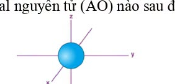
\includegraphics[width=3.8cm]{images_gk1_10_5001/cau9_orbital_s.png}
\end{center}
\choice
{$p_x$.}
{$p_z$.}
{\True s.}
{$p_y$.}

\end{ex}

\begin{ex}
Phát biểu nào sau đây đúng về chu kì 3 trong bảng tuần hoàn các nguyên tố hóa học?
\choice
{bắt đầu từ nguyên tố có $Z = 19$ và kết thúc ở nguyên tố có $Z = 36$.}
{bắt đầu từ nguyên tố có $Z = 11$ và kết thúc ở nguyên tố có $Z = 19$.}
{\True bắt đầu từ nguyên tố có $Z = 11$ và kết thúc ở nguyên tố có $Z = 18$.}
{bắt đầu từ nguyên tố có $Z = 3$ và kết thúc ở nguyên tố có $Z = 10$.}

\end{ex}

\begin{ex}
Cho mô hình cấu tạo nguyên tử như sau:
\begin{center}
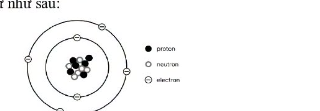
\includegraphics[width=5.5cm]{images_gk1_10_5001/cau11_mo_hinh_nguyen_tu.png}
\end{center}
Kí hiệu đúng của nguyên tử này là
\begin{center}
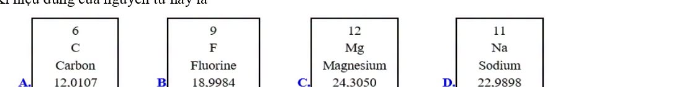
\includegraphics[width=13.5cm]{images_gk1_10_5001/cau11_o_nguyen_to.png}
\end{center}
\choice
{\True Ô số 6 (Carbon -- C).}
{Ô số 9 (Fluorine -- F).}
{Ô số 12 (Magnesium -- Mg).}
{Ô số 11 (Sodium -- Na).}

\end{ex}

\begin{ex}
Hợp kim cobalt được dùng rộng rãi trong động cơ máy bay vì có độ bền cao ở nhiệt độ cao. Nguyên tử cobalt có cấu hình electron lớp ngoài cùng là $3d^74s^2$. Ở trạng thái cơ bản, số electron độc thân trong nguyên tử cobalt là
\choice
{5.}
{2.}
{7.}
{\True 3.}

\end{ex}

\Closesolutionfile{ans}

\vspace{5pt}
\noindent
\textbf{\color{mainGreen}PHẦN II. Câu hỏi trắc nghiệm đúng sai.}\\
\textit{Thí sinh trả lời từ câu 1 đến câu 2. Trong mỗi ý a), b), c), d) ở mỗi câu thí sinh chọn đúng hoặc sai. (2,0 điểm)}

\begin{ex}
Đồng thau là hợp kim của hai kim loại, được dùng để làm van nước, ổ khóa, tay nắm cửa và các nhạc cụ kèn đồng nhờ bền, dễ gia công và ít bị ăn mòn. Kết quả phân tích phổ khối lượng một mẫu đồng thau cho thấy mẫu chứa bốn loại nguyên tử chính X, Y, Z, T với thông tin như sau:
\begin{center}
\begin{tabular}{|c|c|c|c|}
\hline
\textbf{Nguyên tử} & \textbf{Số proton} & \textbf{Số neutron} & \textbf{Tỉ lệ số nguyên tử trong tự nhiên (\%)} \\
\hline
X & 29 & 34 & 69,15 \\
\hline
Y & 30 & 36 & 27,7 \\
\hline
Z & 29 & 36 & 30,85 \\
\hline
T & 30 & 34 & 49,2 \\
\hline
\end{tabular}
\end{center}
\begin{center}
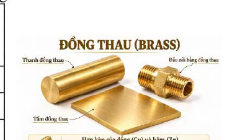
\includegraphics[width=6.5cm]{images_gk1_10_5001/p2_cau1_dong_thau.png}
\end{center}
\choiceTF
{X và T có cùng số neutron nên là đồng vị của nhau}
{\True Bốn loại nguyên tử trong bảng thông tin trên thuộc hai nguyên tố hóa học}
{\True Nguyên tử khối trung bình của nguyên tố tạo nên X là 63,6 (làm tròn kết quả đến hàng phần mười)}
{Nguyên tử khối trung bình của nguyên tố tạo nên T được tính bằng biểu thức $\dfrac{64 \times 49,2 + 66 \times 27,7}{100}$}

\end{ex}

\begin{ex}
Một học sinh hỏi chatbot AI: ``Mô hình nguyên tử hiện đại khác mô hình Rutherford -- Bohr như thế nào?'' Chatbot đưa ra các ý sau về mô hình nguyên tử hiện đại:
\begin{center}

\includegraphics[width=6.5cm]{images_gk1_10_5001/p2_cau2_chatbot_ai.png}
\end{center}
\choiceTF
{Trong mô hình hiện đại, electron chuyển động trên các quỹ đạo tròn có bán kính xác định quanh hạt nhân}
{\True Orbital nguyên tử là vùng không gian xung quanh hạt nhân mà xác suất tìm thấy electron khoảng 90\%}
{Mọi orbital đều có dạng hình cầu, chỉ khác nhau về kích thước}
{\True Mỗi orbital chứa tối đa 2 electron và hai electron này có chiều tự quay ngược nhau}

\end{ex}

\vspace{5pt}
\noindent
\textbf{\color{mainGreen}PHẦN III. Trắc nghiệm trả lời ngắn.}\\
\textit{Học sinh trả lời từ câu 1 đến câu 4. (2,0 điểm)}

\begin{ex}
Khối lượng của một nguyên tử magnesium là $39,8271 \cdot 10^{-27}\text{ kg}$. Biết $1\text{ amu} = 1,6605 \cdot 10^{-27}\text{ kg}$. Khối lượng nguyên tử magnesium tính theo đơn vị amu là bao nhiêu? \textit{(Kết quả làm tròn đến hàng đơn vị.)}
\newline\textbf{Trả lời:} \dotfill
\end{ex}

\begin{ex}
Cho các phát biểu sau:\\
(1) Điện tích của proton và electron có cùng độ lớn nhưng ngược dấu.\\
(2) Có những nguyên tử không chứa neutron nào.\\
(3) Khối lượng nguyên tử hầu hết tập trung ở hạt nhân nguyên tử.\\
(4) Điện tích của proton và neutron có cùng độ lớn nhưng ngược dấu.\\
(5) Khối lượng của proton và neutron xấp xỉ bằng nhau và lớn hơn nhiều khối lượng của electron.\\
Hãy sắp xếp các phát biểu \textbf{không đúng} trong các phát biểu trên theo số thứ tự tăng dần (ví dụ 12, 134, \dots)
\newline\textbf{Trả lời:} \dotfill
\end{ex}

\begin{ex}
Nguyên tử của nguyên tố X có tổng số electron trên các phân lớp p là 11. Số hiệu nguyên tử của X là bao nhiêu?
\newline\textbf{Trả lời:} \dotfill
\end{ex}

\begin{ex}
Dựa vào bảng tuần hoàn các nguyên tố hóa học, cho thông tin về nguyên tố X như sau:
\begin{center}
\begin{tabular}{|c|c|c|c|c|}
\hline
\textbf{Kí hiệu} & \textbf{Số hiệu nguyên tử} & \textbf{Cấu hình e lớp ngoài cùng} & \textbf{Chu kì} & \textbf{Nhóm} \\
\hline
X & 12 & $3s^2$ & 3 & IIA \\
\hline
\end{tabular}
\end{center}
Nguyên tố Y thuộc cùng chu kì với X và thuộc nhóm VIIA. X và Y kết hợp với nhau tạo thành hợp chất có công thức \ce{XY2}. Tổng số proton có trong một phân tử \ce{XY2} là bao nhiêu?
\newline\textbf{Trả lời:} \dotfill
\end{ex}

\vspace{5pt}
\noindent
\textbf{\color{mainGreen}PHẦN IV. TỰ LUẬN.}\\
\textit{HỌC SINH LÀM RA GIẤY THI TRẢ LỜI TỪ CÂU 1 ĐẾN CÂU 3 (3,0 điểm)}

\begin{ex}
\textbf{(0,5 điểm)} Nguyên tố chlorine (\ce{Cl}) có nguyên tử khối trung bình là 35,5. Biết chlorine gồm hai đồng vị bền là \ce{^{35}Cl} và \ce{^{37}Cl}. Để xác định phần trăm các đồng vị bền của chlorine trong tự nhiên, người ta dùng phương pháp phổ khối lượng.\\
\textbf{a)} Hãy xác định phần trăm mỗi đồng vị bền của chlorine. \textit{(0,25 điểm)}\\
\textbf{b)} Hãy cho biết hình ảnh phổ khối lượng nào sau đây của chlorine là phù hợp nhất? Vì sao? \textit{(0,25 điểm)}
\begin{center}
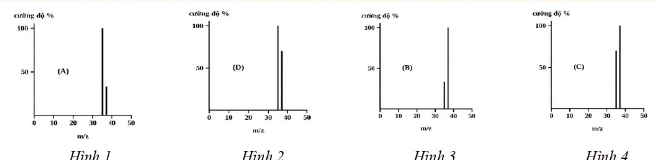
\includegraphics[width=13.5cm]{images_gk1_10_5001/p4_cau1_pho_khoi_luong.png}
\end{center}

\end{ex}

\begin{ex}
\textbf{(0,5 điểm)} Các đám mây gây hiện tượng sấm sét được tạo nên bởi những hạt nước nhỏ li ti mang điện tích. Một phép đo thực nghiệm cho thấy một giọt nước hình cầu có đường kính $5 \cdot 10^{-3}\text{ cm}$ mang điện tích âm là $-3{,}220 \cdot 10^{-17}\text{ C}$. Điện tích âm này là do giọt nước nhận thêm electron.\\
Số phân tử nước trong giọt nước được tính theo biểu thức:
\[
N_{\ce{H2O}} = \dfrac{4}{3} \cdot 3{,}14 \cdot r^3 \cdot \dfrac{D}{18} \cdot N_A
\]
Trong đó $D\text{ (g/cm}^3\text{)}$ là khối lượng riêng của nước, $r\text{ (cm)}$ là bán kính của giọt nước. Biết khối lượng riêng của nước là $1\text{ g/cm}^3$; điện tích của một electron là $-1{,}602 \cdot 10^{-19}\text{ C}$; số Avogadro $N_A = 6{,}022 \cdot 10^{23}\text{ mol}^{-1}$.\\
\textbf{a)} Tính số phân tử nước trong giọt nước. \textit{(0,25 điểm)}\\
\textbf{b)} Trung bình cứ $x \cdot 10^{12}$ phân tử nước có trong giọt nước thì có 1 hạt electron dư. Tính giá trị của $x$ \textit{(Kết quả làm tròn đến hàng đơn vị).} \textit{(0,25 điểm)}

\end{ex}

\begin{ex}
\textbf{(2,0 điểm)} Năm 2019 được chọn là Năm Quốc tế Bảng tuần hoàn các nguyên tố hóa học, kỉ niệm 150 năm Dmitri Ivanovich Mendeleev công bố bảng tuần hoàn (1869). Khi xây dựng bảng, Mendeleev đã để trống một số ô và dự đoán tính chất của các nguyên tố chưa được phát hiện. Một trong số đó là ``eka-aluminium'', nguyên tố nằm ngay dưới nhôm trong cùng một nhóm.\\
Năm 1875, nhà hóa học người Pháp Paul-Émile Lecoq de Boisbaudran công bố tìm ra một nguyên tố mới. Nguyên tố này có nhiều tính chất trùng khớp với eka-aluminium, nhưng khối lượng riêng ông đo được lại khác xa giá trị Mendeleev tiên đoán. Mendeleev đề nghị ông đo lại. Kết quả đo lần sau, với mẫu đã được tinh chế, trùng khớp với dự đoán của Mendeleev. Một cách đơn giản để xác định khối lượng riêng của một mẫu kim loại là dùng bình tràn, như minh họa ở Hình 1.
\begin{center}
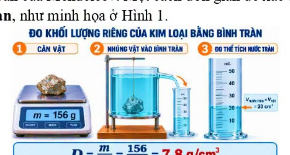
\includegraphics[width=8cm]{images_gk1_10_5001/p4_cau3_binh_tran.png}\\
\textit{\footnotesize Hình 1. Minh họa phương pháp đo khối lượng riêng bằng bình tràn (số liệu trong hình chỉ mang tính minh họa).}
\end{center}
Áp dụng phương pháp này để mô phỏng tái hiện lại phép đo trong lịch sử, một nhóm học sinh cân một mẫu kim loại M (ở $20^\circ\text{C}$) được khối lượng \textbf{35,46 g}. Sau đó, các em thả nhẹ mẫu vào một bình tràn chứa đầy nước và thu được \textbf{6,00 mL} nước tràn ra ống đong. Cho bảng số liệu sau:
\begin{center}
\begin{tabular}{|l|c|c|c|c|c|}
\hline
\textbf{Kim loại} & \textbf{Mg} & \textbf{Al} & \textbf{Cu} & \textbf{Zn} & \textbf{Ga} \\
\hline
Số hiệu nguyên tử (Z) & 12 & 13 & 29 & 30 & 31 \\
\hline
Khối lượng riêng ($\text{g/cm}^3$) & 1,74 & 2,70 & 8,96 & 7,13 & 5,91 \\
\hline
\end{tabular}
\end{center}
\textbf{a)} Tính khối lượng riêng của mẫu kim loại M. Dựa vào bảng số liệu, cho biết M là kim loại nào? \textit{(0,25 điểm)}\\
\textbf{b)} Viết cấu hình electron của nguyên tử M. \textit{(0,25 điểm)}\\
\textbf{c)} Xác định vị trí của M trong bảng tuần hoàn (ô, chu kì, nhóm). \textit{(0,5 điểm)}\\
\textbf{d)} M là nguyên tố s, p, d hay f? \textit{(0,25 điểm)}\\
\textbf{e)} Nguyên tử M có bao nhiêu electron hóa trị? \textit{(0,25 điểm)}\\
\textbf{f)} Dựa vào vị trí của M và Al trong bảng tuần hoàn, hãy cho biết tính chất hoá học của M và Al có tương tự nhau hay không? Vì sao? \textit{(0,25 điểm)}\\
\textbf{g)} Biết nguyên tố In ($Z = 49$) nằm cùng nhóm với nguyên tố nhôm, ngay phía dưới nguyên tố ``eka-aluminium''. Hãy xác định số electron hoá trị của In? \textit{(0,25 điểm)}

\end{ex}

\begin{center}
\textbf{--- HẾT ---}
\end{center}

\end{document}
